% Created 2019-01-10 Do 16:47
% Intended LaTeX compiler: pdflatex
\documentclass[11pt, a4paper]{article}
\usepackage[utf8]{inputenc}
\usepackage[T1]{fontenc}
\usepackage{graphicx}
\usepackage{grffile}
\usepackage{longtable}
\usepackage{wrapfig}
\usepackage{rotating}
\usepackage[normalem]{ulem}
\usepackage{amsmath}
\usepackage{textcomp}
\usepackage{amssymb}
\usepackage{capt-of}
\usepackage{hyperref}
\usepackage[backend=biber, authordate, ibidtracker=context,natbib,doi=false,isbn=false,url=false]{biblatex-chicago}
\usepackage{setspace}
\usepackage{tikz}
\addbibresource{~/Documents/bibliography/references.bib}
\usetikzlibrary{bayesnet} \onehalfspacing
\author{Conrad Friedrich}
\date{\today}
\title{What Bayesian Models of Cognition Tell Us About the Problem of Induction\\\medskip
\large 4457 words}
\hypersetup{
 pdfauthor={Conrad Friedrich},
 pdftitle={What Bayesian Models of Cognition Tell Us About the Problem of Induction},
 pdfkeywords={},
 pdfsubject={},
 pdfcreator={Emacs 26.1 (Org mode 9.1.13)}, 
 pdflang={English}}
\begin{document}

\maketitle

\thispagestyle{empty}

\section{Introduction}
\label{sec:orgd225fbe}

In this paper, we argue that Bayesian models of cognitive processes can help
explicate the inductive bias of a rational reasoner and can thus be employed to
address the age-old problem of induction. In particular, hierarchical Bayesian
models (HBMs) give insight into the structural features of rational inductive
bias. Their use is independently motivated for multiple reasons: HBMs are used
successfully in the cognitive sciences to explain many forms of reasoning. As we
show in this paper, they also naturally account for intuitions about the
rational reasoning in simple and straightforward cases. In addition, HMBs give a
convincing account of why and how inductive biases are formed, when interpreted
as making salient the structure of analogical reasoning as a means to inform
inductive bias in inferences.

What exactly is meant by the `problem of induction'?
\textcite{lipton04_infer_best_explan} notes that in almost all cases, the
available evidence deductively underdetermines deciding between alternative
hypotheses, and argues that additional mechanisms have to be employed to reach a
judgment. He distinguishes between the challenge of \textit{describing} how
these judgments are made in scientific and quotidian situations and the
challenge of \textit{justifying} a given method to reach a judgment. Both kinds
are relevant for the present paper, as we are developing how insight into the
problem of description---as in the computational cognitive sciences---might
inform the problem of justification, which we are particularly interested in
from a philosophical perspective. For the purpose of this paper, we take it that
a justified inference speaks in favor of the truth of its conclusion, for
example as the result produced by a reliable method or by evidential
confirmation.

The problem of induction has been historically pervasive, starting with Hume's
famous argument for the claim that there is no hope for justification of
inferences which go beyond the observed data, as any justification for an
inductive inference must presuppose the validity of inductive inferences
\citep{hume39_treat_human_natur,hume48_enquir_concer_human_under}. In
statistical learning theory,
\citet{wolpert96_lack_prior_distin_between_learn_algor} is said to have
reformulated the problem in formally precise terms in form of the so-called No
Free Lunch theorem. Since reasoning in artificial intelligence, human cognition,
and even the sciences is fundamentally inductive, the problem continues to be
relevant. Many authors (e.g. \citet{vapnik95_natur_statis_learn_theor}) suggest
that a key to successful inductive inference lies in appropriately limiting the
hypotheses under consideration, that is, making use of inductive \emph{biases},
\emph{constraints}, or \emph{priors} \citep{griffiths09_connec}.

The Bayesian framework has already been employed to address the problem of
induction, perhaps most notably in the project of inductive logic
\citep{carnap50_logic_found_probab}. Here too, however, the need for empirical
premises in the form inductive biases became apparent
\citep{henderson18_probl_induc}, in that almost any conclusion can inductively be inferred from the same
set of premises, if the prior belief aren't appropriately restricted.

Studying inductive biases, then, goes a long way in addressing the problem of
justifying inductive inferences. By taking a closer look at successful inductive reasoners and
learning about their inductive biases, we might get informed about the
structure of inductive biases more generally, if not at least get a good idea of
how inductive biases might be acquired and applied. Actual human reasoning is
arguably very successful, and the field of computational cognitive science
builds mathematical models to explain this success
\citep{tenenbaum11_how_to_grow_mind,griffiths10_probab_model_cognit}.

In this paper, we are particularly concerned with the \emph{hierarchical
  structure} of models in cognitive science. We examine how the structure of
these models imposes certain constraints on the learner which induce systematic
inductive biases and give a plausible account of how the biases are acquired.

While there may be no universal learning algorithm, Bayesian models of cognition
indicate what optimal bias could look like. By employing hierarchical
representations, information is learned on different levels of abstraction. A
single learning problem can inform different levels of abstraction, and abstract
knowledge can be transferred to other learning problems, providing biases for
future learning problems.

We argue that hierarchical Bayesian models (HBMs) as used in describing human
inference processes in the cognitive sciences can inform the philosophical
discussion on the problem of induction.

In the cognitive sciences, HBMs bring the virtues of precise formal analysis in
the Bayesian framework to bear on the research modeling biases in inductive
inference processes. They force the researcher to be explicit and precise about
modeling the learner's abstract background knowledge. Bayesian models of human
cognition, and in particular hierarchical models, give a convincing explanation
for the structure and the origin of such inductive biases. By examining these
models closely, we can gain insight into how the biases are formed and updated
and how they contribute to successful inductive inference.

In many situations, human reasoning is an exemplar of successful generalization.
By examining plausible descriptive formal models of inductive bias in successful
reasoning, the philosophical discussion can benefit by identifying key
conditions of a successful inductive inference. We argue for this by---step by
step---building up a more and more complex model of a simple reasoning process,
intending to make transparent the benefits that come with explicitly modeling
inductive bias in the form of abstract hierarchical background knowledge.

The paper is structured as follows. In Section \ref{sec:org873c88f}, we survey
some literature in the cognitive sciences and establish the success of HBMs in
empirical models. Section \ref{sec:orga764b3c} is the main part of the paper. We
develop a hierarchical model for a simple inference problem from the ground up
and look closely at its features. We identify central such features which
contribute to modeling inductive bias with HBMs and emphasize how they support
the claim of the paper. In Section \ref{sec:org87d755f}, finally, we look at
some salient objections and argue against them. Throughout, we took great care
not to get lost in formal detail, while still striving for precise language and
notation.

\section{Hierarchical Bayesian Models of Cognition}
\label{sec:org873c88f}

In this section, we survey some literature in the cognitive science and establish
the success of HBMs in empirical models.

How does the mind get so much from so little? Ask
\citet{tenenbaum11_how_to_grow_mind} pointedly. Their research focuses on issues
in learning and inductive inferences in human cognition, paying particular
attention to the human mind's ability to generate a rich, structured
representation of the world that goes far beyond the limited data available to
the learner. For example, children learn the application of words a lot faster
and with fewer examples than a learner which considers all logically possible
hypotheses, indicating that they employ strong inductive biases limiting the
hypotheses under consideration. A key insight is that the hypotheses are
constrained by abstract knowledge the learner applies to the problem. There are
similarities between different learning problems a learner encounters in her
development. These similarities can often be represented in the form of more
abstract information than the mere data of a problem provides. Learning about one
problem, then, also informs the more abstract level, and facing another,
slightly similar problem, the learner transfers her newly found knowledge in the
form of inductive bias.

Bayesian modeling is a popular way to formally deal with reasoning under
uncertainty, though by no means the only or only popular alternative among other
formalisms \citep{halpern03_reason_about_uncer}. Bayesian models tend to be
semantically transparent and readily interpretable. Hierarchical Bayesian models
(HBM) have been applied to a lot of different learning scenarios, and are
generally found to agree with empirical data. That is, cases of actual human
reasoning can be modeled adequately within the framework in a wide range of
circumstances.\footnote{Many papers cited in this paper provide evidence for this
  claim. Helpful overviews are given by, e.g.
  \citet{tenenbaum06_theor_based_bayes_model_induc_learn_reason,griffiths10_probab_model_cognit,tenenbaum11_how_to_grow_mind}}

What are the elements of the hierarchy? On different levels of the hierarchy are
different types of hypotheses. For example, when modeling language
comprehension, we might use parse trees to model individual sentences. One level
higher, they can be explained by grammars, which in turn might be explained by
recourse to Universal Grammar
\citep{kemp07_learn_overh_with_hierar_bayes_model}. In general, the models are
set up such that we find an explanatory relation between hypotheses on different
levels of the hierarchical model. By additionally supplying probability
distributions with appropriate parameters, this hierarchical structure is
amenable to Bayesian analysis.

Of course, the adequacy of the framework is not without its critics in cognitive
science \citep{mcclelland10_approac_lettin} and in philosophy of cognitive
science \citep{colombo16_bayes_cognit_scien_monop_neglec_framew}, but this
discussion is more general and leads too far afield for the purposes of this
paper.

\section{Modeling Inductive Biases}
\label{sec:orga764b3c}

The section is structured as follows. We first build a simple Bayesian model in
Section \ref{sec:orgcc8b92d} and extend it to a slightly more complex Bayesian
model in Section \ref{sec:org26216a1}. Recognizing and highlighting its
shortcomings, we develop a hierarchical Bayesian model that addresses these
problems in Section \ref{sec:org261bd27}. We examine closely \emph{why} this is
successful and identify structural features that contribute to its
success\footnote{The present section draws on \citet{kruschke11_doing_bayes},
  chapters 5 and 9, \citet{jaynes03_probab_theor}, chapter 6,
  \citet{gelman13_bayes_data_analy_third_edition}, chapter 5, and reproduces a
  model of \citet{kemp07_learn_overh_with_hierar_bayes_model}.}.
\subsection{The Simplest Bayesian Model}
\label{sec:orgcc8b92d}

For the purposes of highlighting different model structures, we take a look at
one of the simplest cases of Bayesian inferences. Following that, we will look
at a model with a slightly more complicated structure.

Consider the oft-used case of estimating the underlying parameter of a
repeatable experiment with dichotomous outcomes. For example, we repeatedly draw
marbles from a bag. We know there are only two different types of marbles, say
blue and white, in the bag. Let's denote the proportion of white marbles in the
bag as \(\theta \in (0,1)\), which is also the probability to draw a white
marble at random. Let \(p\) be a probability distribution over a suitable
measurable space representing our prior beliefs. Given data \emph{y}, which
denotes observed draws \emph{N} with \emph{z}
white marbles, what is our posterior subjective probability about the
proportion? To calculate, we employ Bayes theorem:

\begin{equation}
  p(\theta|y) = \frac{p(y|\theta) p(\theta)}{p(y)}
\end{equation}

where

\begin{equation}
  p(y) = \int p(y|\theta')p(\theta')d\theta'.
\end{equation}

We may plausibly assume each draw generated by a Bernoulli distribution, hence
the likelihood \(p(y|\theta)\) for \(z\) out of \(N\) white marbles is given by the binomial distribution

\begin{equation}
  p(y|\theta) =\binom{N}{z} \theta^z (1-\theta)^{N-z}.
\end{equation}

Lastly, \(p(\theta)\) represents our prior belief of the proportion of white
marbles. In the Bayesian framework, the background knowledge the learner applies
to the problem is represented by the prior belief. The inductive bias of a
learner can be seen as her background knowledge. For the current example, we assume a
prior biased towards uniformity of the bags, as can be seen in Figure
\ref{fig:org759eaed}, top. Formally, we say that \(\theta\) is beta distributed
with parameters \(a,b\):

\begin{equation}
  \theta \sim ~ \text{Beta}(a,b)
\end{equation} 

and set \(a=b=0.5\). Note that this is an arbitrary choice. In the Bayesian
framework, we could use almost any kind of prior as long as it is a probability
distribution.

\begin{figure}[htbp]
  \centering \includegraphics[width=1\linewidth]{./SimpleBayes.pdf}
  \caption{\label{fig:org759eaed} Plots of the model described in Section
    \ref{sec:orgcc8b92d}. Expected values of the posteriors plotted as a
    straight line. Labels for the y-axis omitted.}
\end{figure}

Suppose we draw a single white ball and update our beliefs. The resulting
posterior probability as just defined is plotted in Figure \ref{fig:org759eaed},
center. Our confidence, so to speak, has
shifted from previously high confidence in an all-white and all-blue bag to just
high confidence in an all-white bag. All other proportions of marbles in the bag
are still on the table, however. This posterior is still \emph{vague}.

After observing 20 draws of which 17 have been white, the resulting
posterior is a lot more \emph{certain}, plotted in Figure \ref{fig:org759eaed},
bottom. The data has had considerable impact on the posterior, while the prior
belief does not have much effect. Almost all confidence lies between 0.6 and
1.0. Note that the previously high confidence in an all-white bag is gone.
Pressed for a point estimate of the probability that the next draw is a white
marble, the Bayesian reasoner might give the expected value of the posterior
distribution, plotted as a straight line.

This straightforward problem can be regarded as convincingly addressable in the Bayesian
framework.

\subsection{Multiple Parameters}
\label{sec:org26216a1}

Consider now a case where you encounter a whole stack of bags of marbles. We
open up several bags and find mixed quantities of blue and white marbles. What
can we predict for subsequent draws?

Arguably, the probability of colors drawn from each bag is determined by the
proportion of colors in each bag, and hence an appropriate model has multiple
parameters \(\theta_i\), one for each bag \emph{i}. Since each bag is different,
our prior assumes the bags proportions to be independent from one another, formally \({
  p(\theta_i) = p(\theta_i|\theta_j) }\) for all \(i,j\). We assume the same
prior as before, such that each \(\theta_i \sim \text{Beta}(a,b)\) with
\(a=b=0.5\). Each \(\theta_i\) is individually estimated by the marbles we drew
out of that bag \emph{i}.

Suppose now that we examine 20 bags, of which we draw 20 marbles each. The
results are varied, with the average proportion of white marbles in a bag
tending towards less than \(0.5\). When we decide to open a 21st bag and draw a
white marble, what is the posterior estimate for the proportion in that bag,
i.e. \(p(\theta_{21})\)? It is the same as in the case with only one bag, with
\(N=1, z=1\), Figure \ref{fig:org759eaed}, center. We haven't learned anything
about bag 21 by looking at any of the other bags, per assumption of the model.

This seems unproblematic, so far. Compare, however, your intuition in the
following case:

\begin{description}
\item[{The Uniform Marble Case}] You encounter an abandoned stack of bags of
  marbles, and, out of curiosity, start drawing from one after the other. After
  20 marbles each from 20 bags, all of the marbles have been completely uniform
  in color: 10 bags have been all-blue, 10 have been all-white. You open the
  21st bag, and draw a white marble. What color do you expect the rest of the
  marbles in the bag to be?
\end{description}

The intuition is clear, we claim: We have good reason to assume the rest of the
marbles to be white, therefore we place high confidence on an all-white bag.
More confidence, at least, than would the 21st bag have been the first bag to
open. This intuition is central to the following argument. Let us look at what
our simple model with multiple parameters suggests, as can be seen in Figure
\ref{fig:org4e70fe9}.

\begin{figure}[htbp]
  \centering \includegraphics[width=1.1\linewidth]{./Flat20Bags.pdf}
  \caption{\label{fig:org4e70fe9} Plots from the model described in Section
    \ref{sec:org26216a1}. Each row shows the distributions of a single parameter
    given different data, here \(\theta_1, \theta_{11}, \theta_{21}\). The first
    column shows the priors. The second column shows the posteriors after mixed
    input, where \(N_1 = 20, z_1 = 1, N_{11} = 20, z_{11} = 6, N_{21} = 1,
    z_{21} = 1\). The third column shows the posteriors after observing the
    uniform bags as, where \(N_1 = 20, z_1 = 20, N_{11} = 20, z_{11} = 0, N_{21}
    = 1, z_{21} = 1\).}
\end{figure}

The first two rows show \(\theta_1, \theta_{11}\). Each bag number 1--20 got 20
draws, with different posteriors dependent on the number of white marbles. The
third row shows \(\theta_{21}\), which we estimate after only a single draw as
in uniform marble case. Notably, both posteriors distributions are identical.
They are also identical to the case of a single parameter as described in
Section \ref{sec:orgcc8b92d}. That is, these models do not make any difference
between the cases as far as \(\theta_{21}\) is concerned. The clear intuition
just described suggests that we have stronger confidence in the next marble
drawn from bag 21 being white in the uniform case than in the mixed bag case.
The model as presented cannot account for this intuition.

An immediate response to this challenge is that the modeling assumption is just
wrong: Our prior assumes independent bags, but we clearly reason as if the bags
are not independent. This is certainly right, but giving up the independence
assumption leaves us without a way of determining the posterior distribution,
since we do not know how to calculate the likelihoods. As we will see,
hierarchical models provide a structured way of reasoning about these dependencies. 
In the next section, we'll develop our model further into a
simple hierarchical structure and show how the adjusted model can deal with the
challenge.

\subsection{Introducing Hierarchy}
\label{sec:org261bd27}

Strictly speaking, the model discussed so far already has a hierarchy: We take
the observable data as generated by a parameter \(\theta\) which we cannot directly
observe. Instead, we estimate the parameter. In hierarchical models, we just add
more of these unobserved variables: We take parameter \(\theta\) to be
influenced by additional parameters. Such structures of probabilistic dependence
and independence combined with probability distributions over them can represent
abstract knowledge (e.g.
\cite{goodman11_learn_theor_causal,kemp09_struc_statis_model_induc_reason}). For
example, we might learn in the uniform bags case that the bags tend to be
uniform in color, but that it is not clear whether uniformly blue or white. This
abstract knowledge can be represented by a joint probability distribution over
higher level parameters \citep{kemp07_learn_overh_with_hierar_bayes_model}, as
we will describe and examine in this section.

As before, we observe 21 bags, their data denoted \(y_i\), with parameters
\(\theta_i\). Now, instead of priors with fixed parameters for \(\theta\), we model
the parameters, too. Figure \ref{fig:bayesnet} shows the independency structure.

\begin{figure}[ht]
  \begin{center}
    \begin{tabular}{cc}

      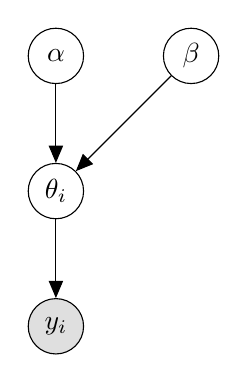
\begin{tikzpicture}

        \node[obs] (y) {$y_i$}; \node[latent, above=of y] (t) {$\theta_i$};
        \node[latent, above=of t] (a) {$\alpha$}; \node[latent, right=of a] (b)
        {$\beta$};

        \edge {t} {y}; \edge {a,b} {t} ;

      \end{tikzpicture}

    \end{tabular}
  \end{center}
  
  \caption{\label{fig:bayesnet} Dependencies intended in the hierarchical model,
    here in form of a directed acyclic graph.}
\end{figure}

In addition to Figure \ref{fig:bayesnet}, the model is given by the following
description.

\begin{align*}
  y_i &\sim \text{Bin}(\theta) \\
  \theta &\sim \text{Beta}(a,b),  \\
  a &= \alpha\beta, \\ 
  b &= \alpha(1-\beta) \\ 
  \alpha &\sim \text{Exp}(1) \\
  \beta &\sim \text{Beta}(1,1) 
\end{align*}

The parameters \(\alpha\) and \(\beta\) describe how we may think the
\(\theta_i\) are distributed, by way of a beta distribution with parameters
\emph{a,b}. They influence all \(\theta_i\). By learning more about a single
\(\theta\), we may shift our confidence about the generating parameters
\(\alpha\) and \(\beta\). This, in turn, influences our beliefs about different
\(\theta_i\).

Formally, given the graph in Figure \ref{fig:bayesnet} to constrain our
probability distribution, we can state\footnote{This is possible since we set up our
  prior probability distribution such that together with the graph in Figure
  \ref{fig:bayesnet} it satisfies the so-called Markov condition, according to
  which a variable is probabilistically independent of its non-descendants,
  conditioned on its parents (the directly preceding nodes). The Markov
  condition in conjunction with the standard multiplication rule of elementary
  probability theory yields Equation \ref{eq:org62f37ab}.} the the posterior joint
distribution as:

\begin{equation}
  \label{eq:org62f37ab}
  p(y_1,\dots,y_n,\theta_1,\dots,\theta_n,\alpha,\beta) = p(\alpha)p(\beta)\prod_{i=1}^n p(y_i|\theta_i)p(\theta_i|\alpha,\beta)
\end{equation}

\begin{figure}[htbp]
  \centering \includegraphics[width=1.1\linewidth]{./Hierarchical20Bags.pdf}
  \caption{\label{fig:org7eac43f} Plots from the model described in Section
    \ref{sec:org261bd27}. Each row shows the distributions of a single parameter
    given different data, here \(\theta_{11}, \theta_{21}\). The first column
    shows the priors. The second column shows the posteriors after mixed input,
    where \(N_{11} = 20, z_{11} = 6, N_{21} = 1, z_{21} = 1\). The third column
    shows the posteriors after observing the uniform bags, where \(N_{11} = 20,
    z_{11} = 0, N_{21} = 1, z_{21} = 1\).}
\end{figure}


In the end, we are mostly interested in the posterior distribution of the
\(\theta_i\) after learning all data. We can calculate the marginal posterior
for, say, \(\theta_{\text{1}}\) by conditioning the joint posterior in Equation
\ref{eq:org62f37ab} on \(y\) and integrating out all other parameters.

Even for simple models like this one, the equation doesn't easily
admit to an analytical solution, such that we need to apply a numerical
strategy. This can be done by dividing the unit interval into a finite partition
and then calculating each and every point of the multivariate posterior for this
partition, sometimes referred to as grid approximation. This becomes quite time
intensive to compute with a growing number of parameters as the number of points
to calculate explodes, at least before optimization. In recent decades, however,
a family of algorithms have been developed to address these issues. These
so-called Markov Chain Monte Carlo (MCMC)\footnote{A very accessible
  introduction can be found e.g. in \citet{kruschke11_doing_bayes}, chapter 7.}
algorithms have been employed to calculate the posteriors in Figure
\ref{fig:org7eac43f}.

Two things should be noted about the results. First, although the priors on
\(\theta\) are identical between this model and the model in Section
\ref{sec:org26216a1}, the posteriors differ. In the uniform case, for
\(\theta_{\text{1}}\) to \(\theta_{\text{20}}\), the hierarchical model allows
the posteriors to be more opinionated and more certain. This is a result of the
learned abstract knowledge that the bags tend to be uniform in color, resulting
in high confidence that the rest of the marbles drawn from any bag will be of
that same color, too.

Second, unlike the model in Section \ref{sec:org26216a1}, the posterior of
\(\theta_{\text{21}}\) differs between both cases in the mixed and uniform case.
Arguably, in both cases the estimate is a lot better: In particular, the result
in the uniform case shows a strong tendency to expect the next marble out of
bag 21 to be white, in accordance with the intuition about the
uniform marble case.

\subsection{Forming Inductive Bias}
\label{sec:org7d2bfe8}

To put it a bit more generally, a big selling point of HBMs is that they enable
the learner to \emph{transfer} learned knowledge from one learning problem to
another. To be sure, in the presented example case, there are other Bayesian
options to account for the transfer of knowledge about the proportion of marbles
from one bag to the next, for example by introducing more complicated models on
the base level. HBMs, though, give a systematic account of how such a transfer
can, in principle, be achieved. And they potentially do so for arbitrary levels of
abstraction, as in hierarchical nonparametric models \parencite{pmlr-v27-salakhutdinov12a}.

By providing this ability to transfer, HBMs give an astonishingly natural
account of how inductive bias for a particular learning problem is acquired: by
recognizing similarity between problems and transferring learned bias from an
old problem to a new one.

The attentive philosopher will note: This requires an inductive bias on a higher
level, namely that similar problems should be addressed similarly, hence that
knowledge on the object level is transferable. But it also requires a bias for
judging two problems as similar. Doesn't this just push the problem of
justifying inductive bias to a higher level, thereby not solving, but instead
just displacing the problem of induction? We claim that is exactly what is
happening, but that the introduced structure is still benefiting our aim of
explicating inductive bias. It is similar to the advantages that Bayesian models
enjoy over classic statistical models: They force us to be explicit about the
prior information we bring into an inference problem. Similarly, HBMs make
explicit the abstract knowledge involved in inductive reasoning. This way,
Bayesian statistics, just as HBMs in cognitive science, open up their respective
research problems to precise analysis. For the philosopher, analogously, HBMs open up
the possibility to precisely analyze the inductive biases implicit in inductive
reasoning problems, and may in this manner shed light on aspects of the bias
that haven't thus far been the focus of research.

\subsection{Hierarchical Bayesian Models of Cognition}
\label{sec:org47c471a}

The example model given above only shows that HBMs \emph{can} give a convincing
account of abstract knowledge in \textit{some} reasoning process. But this is exactly what
we set out to do: Highlight HBMs as a possible way to model abstract knowledge.
Of course, these cases here are oversimplified. Rarely is data just binary
without predictor variables. The levels of abstraction are almost trivial, and
amount to daunting proportions in realistic scenarios. The claim
that HBMs are a plausible model for many, if not almost all, cases of inductive
reasoning with abstract knowledge is vastly stronger. We refer again to
helpful overviews by, e.g.
\citet{tenenbaum06_theor_based_bayes_model_induc_learn_reason,griffiths10_probab_model_cognit,tenenbaum11_how_to_grow_mind}.
HBMs are extremely flexible and can account for very diverse learning problems,
as has been noted in the introduction. They can account for how such abstract
knowledge is learned and formed, too \citep{kemp10_probab_model_theor_format}.

\section{Objections}

In this section, we will address some natural objections to our claim. 
\label{sec:org87d755f}
\subsection{How Does Adding Parameters Reduce Complexity?}
\label{sec:orga21625a}

Making a model more complicated by adding additional parameters runs counter to
the idea of introducing inductive bias, as these are concepts that are usually
seen to be in opposition to one another, as exemplified in the
bias-complexity-tradeoff problem (e.g.
\cite{shalev-shwartz14_under_machin_learn,harman07_reliab_reason}). Instead, we
might run the risk of overfitting. HBMs are undeniably more complicated than
simple, flat models.

We give two reasons that they nevertheless can still plausibly account for
inductive biases in the intended sense. First, HBMs create a certain effect,
called \emph{shrinkage} in the statistical literature
\citep{kruschke11_doing_bayes}. In our bag example, consider the case of
mixed bags (column 2 in both figures). We note that in the non-hierarchical model (Figure
\ref{fig:org4e70fe9}), the posterior of \(\theta_{21}\) is skewed to the right
quite markedly, indicating a high confidence that the next draw will be white,
too. In the hierarchical model (Figure \ref{fig:org7eac43f}), the posterior of
\(\theta_{21}\) is less extreme, and does not even indicate a preference that a
white ball will be drawn next. The posterior is \textit{constrained} by the
higher level parameters. Thus the model is said to shrink, in general, the range
of estimations. This effect naturally reduces overfitting.

Second, the model applies to more data than a single model would. In the bag
example, we treat all data within the same model with a lot of parameters,
instead of having a separate model for each bag. Additionally, by also modeling
more abstract knowledge, the model is open for more abstract data: receiving
information that stacks of back tend to have the same characteristics, for
example, can inform our model as higher level data, so to speak. By accounting
for more data, the risk to overfit is considerably lowered, as
\cite{perfors11_tutor_introd_to_bayes_model_cognit_devel}, Section 4, address.

Taken together, by applying a single, more complex model to more situations and
hence account for more data, hierarchical models \emph{can} induce biases and
avoid increasing complexity.

\subsection{The Argument Rests on an Intuition}
\label{sec:orgee04e3e}

As hinted at in Section \ref{sec:org26216a1}, the central argument employs
intuition as supporting the argument for the use of HBMs. Given that we are talking
about descriptive models, a case might be made that we are mixing up
methodologies here. Why would our intuition about reasoning in certain scenarios
have any bearing on cognitive empirical \textit{science}?

We respond noting that first, we are not making a descriptive claim. Rather, it
is methodological, and hence may very well be confirmed on the grounds of
intuition. Second,  recourse to intuitions is a standard method in the
philosopher's toolbox. Third, similar
intuitions actually have been found to be shared by test subjects
in empirical studies 
\citep{nisbett83_use_statis_heuris_every_induc_reason}.

\subsection{Human Reasoning Does not imply Rational Reasoning}
\label{sec:org7bba5c8}

Conversely, the point might be made that investigating human reasoning cannot
tell us anything about its justification, as we cannot support a normative claim
with descriptive premises. It provably very often the case that humans do not reason rationally. We might even
find that most human reasoning is not rational.

Yet, our case rests on the judgment
that in some exemplary cases of epistemically justified human reasoning, we can
learn something about the inductive biases the reasoner might employ. By
agreement, this inductive bias led to a `good' inference. We take this as
evidence that rational inductive bias is structured
hierarchically. 

\section{Conclusion}
\label{sec:orgceda257}

By giving a systematic account of how inductive bias can be and plausibly is
successfully acquired in many human learning situations, HBMs inform how,
reasonably, abstract background knowledge can be applied to inductive inference
problems. While of course providing no obvious solution to Hume's original problem of
induction, we certainly gain insight into rationally structured inductive bias
in human reasoning, and lay out a promising way of potentially explicating
inductive bias.

\section{Appendix}
\label{sec:orgce6e5db}

The hierarchical models described in this paper and the results presented have
been implemented with the programming language R and a sampling framework called
JAGS, which implements a type of Gibbs sampling Markov Chain Monte Carlo.
Figures \ref{fig:org4e70fe9} and \ref{fig:org7eac43f} have been generated by 4
Markov chains with 200.000 iterations each. Some minor auxiliary functionality
was used from the accompanying program code of \citet{kruschke11_doing_bayes}.
All source code can be reviewed at the author's git repository under

\url{https://github.com/kurtfritz/bayesian-cognition}

\printbibliography
\end{document}